\section{The Proposed Algorithm}
\label{sec:algorithm}

In this paper, the recursive filter is built by cascaded form.
Thus, the algorithms are all explained based on second order recursive equation.
After that, we will discuss the charateristics of a higher order recursive filter
by cascading the second order sections of different algorithms.

The second order recursive filter has the general form, which is given by

\begin{equation}
    \label{eq:recursive_filter}
    % y[n] = x[n] + b_1x[n-1] + b_2x[n-2] + a_1y[n-1] + a_2y[n-2]
    y_n = x_n + b_1x_{n-1} + b_2x_{n-2} + a_1y_{n-1} + a_2y_{n-2}.
\end{equation}
To compute \eqref{eq:recursive_filter}, the dependency problem, happening where the current output sample $y_n$
requires the past two output samples $y_{n-1}$ and $y_{n-2}$, is the inherent obstacle for parallel processing of recursive filter.
One approach is to computing the recursive equation in vector form by taking the advantage of SIMD. 


\subsection{The Previous Block Filtering Algorithm}

The vector form of \eqref{eq:recursive_filter} can be easily proved and given by

\begin{equation}
    \label{eq:block_filtering}
    % y[n] = x[n] + b_1x[n-1] + b_2x[n-2] + a_1y[n-1] + a_2y[n-2]
    \bm{y}[n] = \bm{H}\bm{x}[n] + \bm{B}\bm{x_p}[n] + \bm{A}\bm{y_p}[n] 
\end{equation}
where $\bm{x}[n] = \left[x_{nM}~x_{nM+1} \cdots x_{(n+1)M-1}\right]^T$ denotes a block of
consecutive input samples starting at $x_{nM}$ in size $M$, as well as $\bm{y}[n]$. 
$\bm{x_p}[n]=\left[x_{nM-2}~x_{nM-1}\right]^T$, $\bm{y_p}[n]=\left[y_{nM-2}~y_{nM-1}\right]^T$ are two vectors 
containing the initial conditions. 
$\bm{H}$, $\bm{B}$ and $\bm{A}$ are three constant matrices of size $M {\times} M$.
$M {\times} 2$ and $M {\times} 2$, 
Specifically, $\bm{H}$ is a lower triangular Toeplitz matrix, where the first
column is the impulse response of the recursive equation, i.e.,

\begin{equation*}
    \bm{H} = \left[\arraycolsep=3.0pt\def\arraystretch{1.2}
        \begin{array}{c:c:c:c:c}
        1 & 0 & \cdots & \cdots & 0 \\ 
        b_1{+}a_1 & 1 & \ddots & 0  & \vdots \\
        a_1b_1{+}b_2{+}a_1^2{+}a_2 & b_1{+}a_1 & 1 & \ddots & \vdots \\
        \vdots & \ddots & \ddots & \ddots & 0 \\
        \vdots & \ddots & \ddots & \ddots & 1 \\
        \end{array}\right].  \\
\end{equation*}
The second columns of $\bm{B}$ and $\bm{A}$ are obtained by partitioning the lagged impulse response,
while the first columns of both matrices show the similar features as the second columns with a 
(non-strict) impulse response, where the beginning impulse skips the first taps 
of $x$ and $y$, and directly go to the second taps. Thus, $\bm{B}$ and $\bm{A}$ are given as follows, 

\begin{equation*}
    \begin{aligned}
          \bm{B} {=} \left[\arraycolsep=1.0pt\def\arraystretch{1.0}
            \begin{array}{c:c}
        b_2 & b_1 \\ 
        a_1b_2 & a_1b_1{+}b_2 \\
        a_1^2b_2{+}a_2b_2 & a_1^2b_1{+}a_1b_2{+}a_2b_1 \\
        \vdots & \vdots \\
        \end{array}\right], 
        \bm{A} {=} \left[\arraycolsep=1.0pt\def\arraystretch{1.0}
            \begin{array}{c:c} 
            a_2 & a_1 \\ 
            a_1a_2 & a_1^2{+}a_2 \\
            a_1^2a_2{+}a_2^2 & a_1^3{+}2a_1a_2 \\
            \vdots & \vdots \\
            \end{array}\right]
        \end{aligned}
\end{equation*}

If we compute \eqref{eq:block_filtering} by SIMD, 
to realize the parallelism as much as possible,
the block size $M$ is normally 
determined to be equal to the largest size of SIMD vector that is supported by the processor.
We use the dashed line inside the above matrices to seperate those by SIMD vectors, 
where the memory of data in the same vector are consecutive.
This procedure makes it easier to figure out how the algorithm is performed by SIMD.
For example, to compute $\bm{B}\bm{x_p}$, we perform two multiplication and additions by the first column of $\bm{B}$ and the first value of $\bm{x_p}$,
then the second column of $\bm{B}$ and the second value of $\bm{x_p}$.

Thus, the computation of \eqref{eq:block_filtering} requires $M+4$ fused multiplication and additions (FMAs).
To be more specific, the number of FMAs are seperated by $M{+}2$ for getting the particular solution, i.e.,
$\bm{H}\bm{x}+\bm{B}\bm{x_p}$, and the rest 2 FMAs are for the homogeneous solution, i.e., $\bm{Ay_p}$.
Furthermore, the number of FMAs for each sample is equal to $1{+}4/M$, 
which approaches 1 when $M$ goes to infinity.
The computing complexity is 1 that is independent of the block length,
which also shows block filtering realizes intra-block parallelism.

% which  
% approaches 1 when $M$ goes to infinity. The computing complexity is $O(1)$ that is independent of the block length. 

\subsection{The Proposed Multi-block Filtering Algorithm}

Compared with the block filtering method, the basic idea of multi-block filtering is to partition the consecutive samples into multiple blocks to exploit more
parallelism between blocks.
In particular, consider a $M {\times} M$ squared matrix of samples, i.e., a combination of $M$ consecutive blocks each with $M$ consecutive samples in the block.
The direct way to seperating the $M^2$ consecutive samples into different blocks is by matrix transpose,
e.g., the matrix version of input samples after matrix transpose is 

\begin{equation*}
    \begin{aligned}
    \bm{X}^T[n] = \left[
        \arraycolsep=1.0pt\def\arraystretch{1.0}
        \begin{array}{c:c:c:c}
        x_{nM^2} & x_{nM^2+1} & \cdots & x_{nM^2+M-1} \\ 
        x_{nM^2+M} & x_{nM^2+M+1} & \cdots & x_{nM^2+2M-1} \\
        \vdots & \vdots & \ddots & \vdots \\
        x_{(n+1)M^2-M} & x_{(n+1)M^2-M+1} &\cdots & x_{(n+1)M^2-1} \\
        \end{array}\right]
    \end{aligned}
\end{equation*}
The memory of adjacent samples after the matrix transpose is seperated by the block length $M$.

Note, for the rest of paper, we omit the global index $n$ for the matrix representation of samples,
instead we only focus on the local index of samples inside the matrix, i.e.,
we only look at $\bm{X}^T {\triangleq} \bm{X}^T[0]$.
By doing this, the notations become easier to recognize and 
we can more focus on the algorithm performing for each matrix of samples.
% By doing this, the notations become easier to recognize and it doesn't affect to understanding
% the algorithms performed for one matrix of samples. 
Furthermore, 
we use $\bm{X}_{[n][m]}$ to denote the $m$th sample at the $n$th block
of matrix $\bm{X}$. Next, we are going to explain how exactly the multi-block filtering algorithm works in this paper. 
% by seperating into solving the particular and homogeneous parts.

\subsubsection{Zero initial condition (ZIC)}

The efficient way of solving the recursive equation in matrix form is to seperately compute
the particular and homogeneous parts. The process of solving the particular part in this paper is called
ZIC since we assume zeroing the initial conditions of the homogeneous part. 
The function of ZIC for computing a transposed matrix of samples is given by

\begin{equation}
    \label{eq:ZIC}
    \begin{aligned}
        &\bm{W}^T = \bm{X}^T 
        + b_2{\left[\arraycolsep=1.0pt\def\arraystretch{1.0}
        \begin{array}{c:c:c:c}
        x_{-2} & x_{-1} & \cdots & x_{M-3} \\ 
        x_{M-2} & x_{M-1} & \cdots & x_{2M-3} \\
        \vdots & \vdots & \ddots & \vdots \\
        x_{M^2-M-2} & x_{M^2-M-1} & \cdots & x_{M^2-3} \\
        \end{array}\right]} + \\ 
        & b_1\left[\arraycolsep=1.0pt\def\arraystretch{1.0}
        \begin{array}{c:c:c:c}
        x_{-1} & x_0 & \cdots & x_{M-2} \\ 
        x_{M-1} & x_M & \cdots & x_{2M-2} \\
        \vdots & \vdots & \ddots & \vdots \\
        x_{M^2-M-1} & x_{M^2-M} & \cdots & x_{M^2-2} \\
        \end{array}\right]
        {+} a_2\left[\arraycolsep=1.0pt\def\arraystretch{1.0}
                \begin{array}{c:c:c:c:c}
                0 & 0 & w_0 & \cdots & w_{M-3} \\ 
                0 & 0 & w_M & \cdots & w_{2M-3} \\
                \vdots & \vdots & \vdots & \ddots & \vdots \\
                0 & 0 & w_{M^2-M} & \cdots & w_{M^2-3} \\
                \end{array}\right] \\
        &+ a_1\left[\arraycolsep=1.0pt\def\arraystretch{1.0}
            \begin{array}{c:c:c:c:c}
            0 & w_0 & w_1 & \cdots & w_{M-2} \\ 
            0 & w_M & w_{M+1} & \cdots & w_{2M-2} \\
            \vdots & \vdots & \vdots & \ddots & \vdots \\
            0 & w_{M^2-M} & w_{M^2-M+1} & \cdots & w_{M^2-2} \\
            \end{array}\right]
    \end{aligned}
\end{equation}
% where $\bm{X_{-1}}^T$ and $\bm{X_{-2}}^T$ represent a shifted version of matrix $\bm{X}^T$, in which the positions of all samples
% in $\bm{X}^T$ are lagged by 1 or 2 with $x_{-1}$ and $x_{-2}$ inserted ahead of samples.

It can be seen that to execute \eqref{eq:ZIC}, two blocks, which contain the initial conditions of the particular part, 
i.e., starting at $x_{-2}$ and $x_{-1}$, should be prepared for computing the first block of $\bm{W}^T$. 
This procedure takes 2 shuffles with the last two blocks of $\bm{X}^T$.
Then, the computations can be sequentially forwarded.
Note that the matrices multiplied by $a_1$ and $a_2$ containing the blocks of $\bm{W}^T$
brings the dependency problem. 
Compared with block filtering,
the inherent dependency of solving the particular part of recursive equation by multi-block filtering
is propagated to samples at every position in block, thus, realizes inter-block parallelism.
The number of FMAs for each sample is reduced to $4/M{-}3/M^2$, which goes to 0 when $M$ is arbitrary large.
The computing complexity is $O(1/M)$, which corres\-ponds to the feature of inter-block parallelism.


% The computing complexity of ZIC is $O(4/M)$, which corresponds to the feature of inter-block parallelism.

\subsubsection{Initial condition correction (ICC)}

After computing the output of ZIC, the next step is to 
correct the initial conditions of the homogeneous part of the recursive equation to get the complete solution.
The function is named ICC and given by

\begin{equation}
    \label{eq:ICC}
    \begin{aligned}
        \bm{Y}^T &= \bm{W}^T + \left[\arraycolsep=1.0pt\def\arraystretch{1.0}
                \begin{array}{c:c}
                y_{-1} & y_{-2} \\ 
                y_{M-1} & y_{M-2} \\
                \vdots & \vdots \\
                y_{M^2-M-1} & y_{M^2-M-2}
                \end{array}\right]  
                \left[\arraycolsep=1.6pt\def\arraystretch{1.0}
                    \begin{array}{cccc}
                    a_1 & a_1^2{+}a_2 & a_1^3{+}2a_1a_2 & \cdots \\ 
                    a_2 & a_1a_2 & a_1^2a_2{+}a_2^2 & \cdots \\
                    \end{array}\right] \\
        & = \bm{W}^T + \bm{Y_p}^T  \bm{A}^T
    \end{aligned}
\end{equation}
where $\bm{Y_p}^T$ denotes a $M{\times}2$ matrix, which includes two blocks of initial conditions for the first block of $\bm{Y}^T$.
The function of ICC in \eqref{eq:ICC} is performed essentially by complementing 
$\bm{W}^T$ of ZIC with initial-condition matrix $\bm{Y_p}^T$ and two impulse response sequences defined in $\bm{A}$.
To compute $\bm{Y_p}^T$, or alternatively, the last two blocks of $\bm{Y}^T$, i.e.,
$\bm{Y}^T_{[M-2]}$ and $\bm{Y}^T_{[M-1]}$,
we first define a length-2 vector $\bm{y_e}$, which contains the samples at the
same position of last two blocks, i.e.,
$\bm{y_e}[n] {=} \left[y_{(n+1)M{-}2} ~ y_{(n+1)M{-}1}\right]^T$, 
as well as $\bm{w_e}$ of the input matrix $\bm{W}^T$.
The relationship between $\bm{y_e}$ and $\bm{w_e}$ can be easily proved and given by

\begin{equation}
    \label{eq:ICC_last_two_blocks}
        \bm{y_e}[n] = \bm{w_e}[n]+\bm{C}\bm{y_e}[n{-}1], ~ \text{for} ~ n=0,1,\cdots, M{-}1
\end{equation}
where $\bm{C}$ is a $2{\times}2$ matrix composed by the elements of $\bm{A}$, i.e.,

\begin{equation*}
    \bm{C} = \left[\arraycolsep=1.0pt\def\arraystretch{1.0}
        \begin{array}{cc}
        \bm{A}_{[0][M-2]} & \bm{A}_{[1][M-2]} \\ 
        \bm{A}_{[0][M-1]} & \bm{A}_{[1][M-1]} \\ 
        \end{array}\right].
\end{equation*}
Thus, we can simply compute $\bm{Y_p}^T$ by sequentially performing \eqref{eq:ICC_last_two_blocks}. 

However, it is indirect to computing $\bm{Y_p}^T$ in SIMD from \eqref{eq:ICC_last_two_blocks} 
since $\bm{y_e}$ (or $\bm{w_e}$) interleaves the samples of $\bm{Y}^T_{[M-2]}$ and $\bm{Y}^T_{[M-1]}$,
i.e., the memory of data in $\bm{y_e}$ (or $\bm{w_e}$) are not consecutive. 
One approach to computing the last two blocks of $\bm{Y}^T$ in SIMD 
is by flattening $\bm{Y}^T_{[M-2]}$ and $\bm{Y}^T_{[M-1]}$
in a longer vector and computing a large matrix multiplication, which is given by

% However, the challenge of computing $\bm{Y_p}^T$ by SIMD directly from \eqref{eq:ICC_last_two_blocks} is
% that $\bm{y_e}$ (or $\bm{w_e}$) interleaves the samples of $\bm{Y}^T_{[M-2]}$ and $\bm{Y}^T_{[M-1]}$.
% One approach to computing the last two blocks of $\bm{Y}^T$ in SIMD is by flattening $\bm{Y}^T_{[M-2]}$ and $\bm{Y}^T_{[M-1]}$
% in a longer vector and computing a large matrix multiplication, i.e.,

\begin{equation*}
    \begin{aligned}
        \left[\arraycolsep=1.0pt\def\arraystretch{1.0}
                \begin{array}{c}
                \bm{Y}^T_{[M-2]} \\ [0.5ex] \hdashline 
                \bm{Y}^T_{[M-1]} \\ 
                \end{array}\right] = \bm{T} \left[\arraycolsep=1.0pt\def\arraystretch{1.0}
                \begin{array}{c}
                \bm{W}^T_{[M-2]} \\ [0.5ex] \hdashline
                \bm{W}^T_{[M-1]} \\ 
                \end{array}\right] + \bm{D} \left[\arraycolsep=1.0pt\def\arraystretch{1.0}
                \begin{array}{c}
                y_{-2} \\  
                y_{-1} \\ 
                \end{array}\right] \\
        % \bm{y_e} = \bm{T} \bm{w_e} + \bm{D}\bm{y_p}
    \end{aligned}
\end{equation*}
where $\bm{T}$ is a constant lower triangular Toeplitz matrix of size $2M {\times}2M$,
and $\bm{D}$ is a $2M {\times} 2$ matrix, in which the elements are related to $\bm{T}$.
However, the problem of this approach is that $\bm{T}$ is oversized.
The matrix multiplication of $\bm{T}$ and the vector of $\bm{W}^T$
has to be computed by $4M$ FMAs because the length of
supported SIMD instructions is restricted by $M$. Thus, we do not explain the details of this approach,
instead we propose a more efficient way to computing 
$\bm{Y_p}^T$, which is based on the idea of recursive doubling \cite{Kogge_73}.













% The challenge of executing \eqref{eq:ICC} is to get $\bm{Y_p}^T$ at the first step,
% meaning we need to compute later outputs before earlier outputs,
% e.g., computing $y_{M-1}$ before $y_0$, which breaks through the inherent dependency of recursive equation.
% However, it can be done since $\bm{Y_p}^T$ is also the initial matrix 
% for the last two blocks of $\bm{Y}^T$ where they share the same samples.
% As a result, one approach to computing $\bm{Y_p}^T$, or alternatively, the last two blocks of $\bm{Y}^T$
% can be performed by the matrix multiplication of the last two blocks of
% $\bm{W}^T$ and a constant matrix plus another matrix multiplication with the initial conditions of the homogeneous part, i.e.,

% \begin{equation*}
%     \begin{aligned}
%         \left[\arraycolsep=1.0pt\def\arraystretch{1.0}
%                 \begin{array}{c}
%                 \bm{Y}^T_{[M-2]} \\ [0.5ex] \hdashline 
%                 \bm{Y}^T_{[M-1]} \\ 
%                 \end{array}\right] = \bm{T} \left[\arraycolsep=1.0pt\def\arraystretch{1.0}
%                 \begin{array}{c}
%                 \bm{W}^T_{[M-2]} \\ [0.5ex] \hdashline
%                 \bm{W}^T_{[M-1]} \\ 
%                 \end{array}\right] + \bm{D} \left[\arraycolsep=1.0pt\def\arraystretch{1.0}
%                 \begin{array}{c}
%                 y_{-2} \\  
%                 y_{-1} \\ 
%                 \end{array}\right] \\
%         % \bm{y_e} = \bm{T} \bm{w_e} + \bm{D}\bm{y_p}
%     \end{aligned}
% \end{equation*}
% where $\bm{T}$ and $\bm{D}$ are two constant matrices of size $2M \times 2M$ and $2M \times 2$
% composed by the last two elements of the two impulse response sequences in $\bm{A}$.
% where $\bm{T}$, $\bm{D}$ are two constant matrices of size $2M \times 2M$ and $2M \times 2$.
% The problem of this method is that $\bm{T}$ is oversized.
% The matrix multiplication of $\bm{T}$ and the long vector of $\bm{W}^T$
% % including the last two blocks of $\bm{W}^T$ 
% has to be computed by $4M$ FMAs 
% % because
% % the largest size of SIMD vector that can be processed is restricted by $M$.
% since the length of supported SIMD instructions is restricted by $M$.
% % Due to the non-efficiency, 
% Thus, we don't explain the details of this method,
% instead we propose a more efficient way to computing 
% $\bm{Y_p}^T$, which is based on the idea of recursive doubling.

\begin{figure}[t]
    \centerline{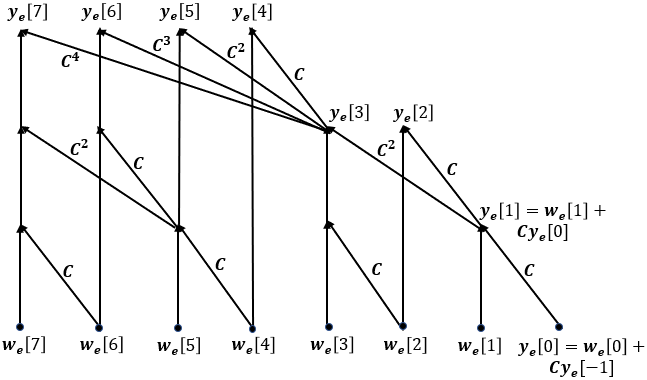
\includegraphics[width=3.3in]{recursive_doubling.png}}
    \caption{Computing the last two blocks of $\bm{Y}^T$ by recursive doubling ($M=8$)}
    \label{fig:Recursive_doubling}
  \end{figure}

The basic idea of recursive doubling method is to split the computation of a function into two equally level of functions,
which can be computed in parallel, and sub-functions are split again and again to increase the degree of parallelism.
Thus, the computating complexity is reduced from $O(M)$ to $O(\log_2M)$.
Figure \ref{fig:Recursive_doubling} illustrates how to compute 8 numbers of $\bm{y_e}$ simulta\-neously
by recursive doubling.
% Figure \ref{fig:Recursive_doubling} illustrates how to compute the last two blocks of $\bm{Y}^T$ by 
% recursive doubling if $M=8$, where $\bm{y_e}$ denotes the vector including two samples at the same position 
% of $\bm{Y}^T_{[M-2]}$, $\bm{Y}^T_{[M-1]}$,
% i.e., $\bm{y_e}[n] = \left[y_{(n+1)M-2} ~ y_{(n+1)M-1}\right]^T$, as well as $\bm{w_e}$.
% % , where $\bm{y_e}$ denotes a vector including the two samples at the same position 
% % of the last two blocks
% % i.e., $\bm{y_e}[n] = \left[y_{(n+1)M-2} ~ y_{(n+1)M-1}\right]^T$, as well as $\bm{w_e}$.
% $\bm{C}$ is a constant matrix
% of size $2 \times 2$ composed by the last two pairs of impulse responses in $\bm{A}$, i.e.,
% \begin{equation*}
%     \bm{C} = \left[\arraycolsep=1.0pt\def\arraystretch{1.0}
%         \begin{array}{cc}
%         \bm{A}_{[0][M-2]} & \bm{A}_{[1][M-2]} \\ 
%         \bm{A}_{[0][M-1]} & \bm{A}_{[1][M-1]} \\ 
%         \end{array}\right].
% \end{equation*}
The accuracy of Figure \ref{fig:Recursive_doubling} can be checked by
$\bm{y_e}[7]$, where

\begin{equation*}
    \begin{aligned}
        \bm{y_e}[7] &= \bm{w_e}[7] + \bm{C}\bm{y_e}[6] \\
        &= \bm{w_e}[7] + \bm{C}(\bm{w_e}[6] + \bm{C}\bm{y_e}[5]) \\
        % &= \bm{w_e}[7] + \bm{C}(\bm{w_e}[6] + \bm{C}(\bm{w_e}[6] + \bm{C}(\bm{w_e}[6] + \bm{C}\bm{y_e}[5])))
        &= \bm{w_e}[7] + \bm{C}\bm{w_e}[6] + \bm{C}^2\bm{w_e}[5] + \bm{C}^3\bm{w_e}[4] + \bm{C}^4\bm{y_e}[3]
    \end{aligned}
\end{equation*}

\begin{algorithm}[t]
    \caption{Computing $\bm{Y_p}^T$ by SIMD and recursive doubling}\label{recursive_doubling}
    \begin{algorithmic}[1]
        \Procedure{Yp\_RD}{$\bm{W}^T[~][~],\bm{C}[~][~],y_{-2},y_{-1}$} 
            \State $\bm{Y}^T_{[M-2]} \gets \bm{W}^T_{[M-2]} + y_{-2}\times \left[\bm{C}_{[0][0]} ~ 0 \cdots 0\right]$ 
            \Statex $ \quad\quad\quad\quad\quad\quad\quad + y_{-1}\times \left[\bm{C}_{[0][1]} ~ 0 \cdots 0\right]$ 
            \State $\bm{Y}^T_{[M-1]} \gets \bm{W}^T_{[M-1]} + y_{-2}\times \left[\bm{C}_{[1][0]} ~ 0 \cdots 0\right]$ 
            \Statex $ \quad\quad\quad\quad\quad\quad\quad + y_{-1}\times \left[\bm{C}_{[1][1]} ~ 0 \cdots 0\right]$ \Comment{Initialization}
            \For{$n \gets 1$ to $\log_2M$}
                \If{$n==1$} 
                    \State $\bm{b_2} \gets $ shuffle $\bm{Y}^T_{[M{-}2]}$: move samples at odd in-
                    \Statex $\quad\quad\quad\quad\quad\quad$ dexes $i$ to $i+1$ and set zeros at odd indexes. 
                    \State $\bm{b_1} \gets $ shuffle $\bm{Y}^T_{[M-1]}$: as above.
                    \State $\bm{Y}^T_{[M-2]} \gets \bm{Y}^T_{[M-2]} {+} \bm{b_{2}}{\times} \left[0 ~ \bm{C}_{[0][0]}\cdots0 ~ \bm{C}_{[0][0]} \right]$ 
                    \Statex $ \quad\quad\quad\quad\quad\quad\quad\quad\quad\quad\quad~~~ + \bm{b_{1}}\times \left[0 ~ \bm{C}_{[0][1]} \cdots 0 ~ \bm{C}_{[0][1]}\right]$ 
                    \State $\bm{Y}^T_{[M-1]} \gets \bm{Y}^T_{[M-1]} {+} \bm{b_{2}}{\times} \left[0 ~ \bm{C}_{[1][0]}\cdots 0 ~ \bm{C}_{[1][0]}\right]$ 
                    \Statex $ \quad\quad\quad\quad\quad\quad\quad\quad\quad\quad\quad~~~ + \bm{b_{1}}\times \left[0 ~ \bm{C}_{[1][1]}\cdots 0 ~ \bm{C}_{[1][1]}\right]$ 
                \ElsIf{$n==2$}
                    \State $\bm{b_2} \gets $ shuffle $\bm{Y}^T_{[M-2]}$: move every second sam-
                    \Statex $\quad\quad\quad\quad\quad~~$ ples at $i$ to $i{+}1$, $i{+}2$ and set zeros at $i$, $i{-}1$.
                    \State $\bm{b_1} \gets $ shuffle $\bm{Y}^T_{[M-1]}$: as above.
                    \State $\bm{Y}^T_{[M-2]} \gets \bm{Y}^T_{[M-2]} {+} \bm{b_{2}} {\times} \left[0 ~ 0 ~ \bm{C}_{[0][0]} ~ \bm{C}^2_{[0][0]}\cdot\cdot \right]$ 
                    \Statex $ \quad\quad\quad\quad\quad~~~ + \bm{b_{1}} {\times} \left[0 ~ 0 ~ \bm{C}_{[0][1]} ~ \bm{C}^2_{[0][1]} \cdots \bm{C}_{[0][1]} ~ \bm{C}^2_{[0][1]}\right]$ 
                    \State $\bm{Y}^T_{[M-1]} \gets \bm{Y}^T_{[M-1]} {+} \bm{b_{2}} {\times} \left[0 ~ 0 ~ \bm{C}_{[1][0]} ~ \bm{C}^2_{[1][0]} \cdot\cdot \right]$ 
                    \Statex $ \quad\quad\quad\quad\quad~~~ + \bm{b_{1}} {\times}  \left[0 ~ 0 ~ \bm{C}_{[1][1]} ~ \bm{C}^2_{[1][1]} \cdots \bm{C}_{[1][1]} ~ \bm{C}^2_{[1][1]}\right]$ 
                    \State \textbf{continue} $\quad\quad\quad\quad~~$ \Comment{follow the above rules}
                    \Statex $\quad\quad\quad\quad\quad\quad\quad\quad\quad\quad\quad\quad~~$ and Figure \ref{fig:Recursive_doubling} to update $\bm{Y}^T$
                \EndIf
            \EndFor
            \State $\bm{Y_p}^T$$_{[0]}$ $\gets $ shuffle $\bm{Y}^T_{[M-2]}$: shift all samples by 1 index
            \Statex $\quad\quad\quad\quad\quad\quad\quad\quad\quad$ and set $y_{-2}$ at the first index.
            \State $\bm{Y_p}^T$$_{[1]}$ $ \gets $ shuffle $\bm{Y}^T_{[M-1]}$: shift all samples by 1 index
            \Statex $\quad\quad\quad\quad\quad\quad\quad\quad\quad$ and set $y_{-1}$ at the first index.            
            \State \textbf{return} $\bm{Y_p}^T$ 
        \EndProcedure
    \end{algorithmic}
\end{algorithm}

Then, we will discuss how Figure \ref{fig:Recursive_doubling} is performed by SIMD.
Because the $M$ number of input $\bm{w_e}[n]$ interleave the samples of $\bm{W}^T_{[M-2]}$ and $\bm{W}^T_{[M-1]}$,
instead of matrix multiplication,
the computation can be partitioned into 4 FMAs by SIMD at each level (recursion). 
Besides that, two shuffles are needed to pre\-pare the vectors of branches for FMAs (per recursion).
Three things should also be noted. Firstly, it takes $\log_2M$ number of recursions.
Then, 4 extra FMAs are needed to initialize the 
computing progress, i.e., to compute $\bm{y_e}[0]$.
Finally, we also need 2 shuffles to get $\bm{Y_p}^T$ for executing \eqref{eq:ICC}.
Thus, the algorithm of calculating
$\bm{Y_p}^T$ by SIMD and recursive doubling is shown in Algorithm \ref{recursive_doubling}. 


% recursion.
% Besides that, two shuffles are needed to prepare the vectors of branches for FMAs (at each recursion). 
% Three things should also be noted. First, the recursive doubling takes totally $\log_2M$ numbers of recursion.
% Second, it needs extra 4 FMAs to initialize the computing progress, i.e., to compute $\bm{y_e}[0]$.
% Finally, after computing the last two blocks of $\bm{Y^T}$, 
% we need 2 shuffles to get $\bm{Y_p}^T$ for executing \eqref{eq:ICC}. 
% The algorithm of calculating $\bm{Y_p}^T$ by SIMD and recursive doubling is shown in Algorithm \ref{recursive_doubling}. 

% Then, we discuss how recursive doubling algorithm can be performed by SIMD.
% It can be seen the $M$ numbers of input $\bm{w_e}[n]$
% essentially interleave the samples of the last two blocks of $\bm{W}^T$.
% Thus, instead of doing the matrix multiplication, the computation can be partitioned into 4 FMAs by SIMD at each
% recursion. Besides that, two shuffles are needed to prepare the vectors of branches for FMAs (at each recursion). 
% Three things should also be noted. Firstly, the recursive doubling algorithm takes totally $\log_2M$ numbers of recursion.
% Secondly, it also needs extra 4 FMAs to initialize the computing progress, i.e., to compute $\bm{y_e}[0]$.
% Lastly, after computing the last two blocks of $\bm{Y^T}$, 
% we need 2 shuffles to get $\bm{Y_p}^T$ for executing \eqref{eq:ICC}. 
% Thus, 
% the algorithm of calculating $\bm{Y_p}^T$ by SIMD and recursive doubling method is shown below 

% \begin{algorithm}
%     \caption{Computing $\bm{Y_p}^T$ by SIMD and recursive doubling}\label{recursive_doubling}
%     \begin{algorithmic}[1]
%         \Procedure{Yp\_RD}{$\bm{W}^T[M][M],\bm{C}[2][2],y_{-2},y_{-1}$} 
%             \State $\bm{Y}^T[M{-}2] \gets \bm{W}^T[M{-}2] + y_{-2}\times \left[\bm{C}[0][0] ~ 0 \cdots 0\right]$ 
%             \Statex $ \quad\quad\quad\quad\quad\quad\quad + y_{-1}\times \left[\bm{C}[0][1] ~ 0 \cdots 0\right]$ \Comment{Initialization}
%             \State $\bm{Y}^T[M{-}1] \gets \bm{W}^T[M{-}1] + y_{-2}\times \left[\bm{C}[1][0] ~ 0 \cdots 0\right]$ 
%             \Statex $ \quad\quad\quad\quad\quad\quad\quad + y_{-1}\times \left[\bm{C}[1][1] ~ 0 \cdots 0\right]$ 
%             \For{$n \gets 1$ to $\log_2M$}
%                 \If{$n==1$} 
%                     \State $b_2 \gets $ shuffle $\bm{Y}^T[M{-}2]$: move values at odd 
%                     \Statex $\quad\quad\quad\quad\quad$ indexes $i$ to $i+1$ and set zeros at odd indexes. 
%                     \State $b_1 \gets $ shuffle $\bm{Y}^T[M{-}1]$: as above.
%                     \State $\bm{Y}^T[M{-}2] \gets \bm{Y}^T[M{-}2] + b_{2}\times \left[0 ~ \bm{C}[0][0]\cdots \right]$ 
%                     \Statex $ \quad\quad\quad\quad\quad\quad\quad\quad\quad\quad + b_{1}\times \left[0 ~ \bm{C}[0][1] \cdots 0 ~ \bm{C}[0][1]\right]$ 
%                     \State $\bm{Y}^T[M{-}1] \gets \bm{Y}^T[M{-}1] + b_{2}\times \left[0 ~ \bm{C}[1][0]\cdots \right]$ 
%                     \Statex $ \quad\quad\quad\quad\quad\quad\quad\quad\quad\quad + b_{1}\times \left[0 ~ \bm{C}[1][1]\cdots 0 ~ \bm{C}[1][1]\right]$ 
%                 \ElsIf{$n==2$}
%                     \State $b_2 \gets $ shuffle $\bm{Y}^T[M{-}2]$: move every second
%                     \Statex $\quad\quad\quad\quad\quad$ values at $i$ to $i{+}1$, $i{+}2$ and set zeros at $i$, $i{-}1$.
%                     \State $b_1 \gets $ shuffle $\bm{Y}^T[M{-}1]$: as above.
%                     \State $\bm{Y}^T[M{-}2] \gets \bm{Y}^T[M{-}2] + b_{2} \left[0 ~ 0 ~ \bm{C}[0][0]\cdots \right]$ 
%                     \Statex $ \quad\quad\quad\quad\quad\quad~~ + b_{1}  \left[0 ~ 0 ~ \bm{C}[0][1] ~ \bm{C}^2[0][1] \cdots \bm{C}^2[0][1]\right]$ 
%                     \State $\bm{Y}^T[M{-}1] \gets \bm{Y}^T[M{-}1] + b_{2} \left[0 ~ 0 ~ \bm{C}[1][0]\cdots \right]$ 
%                     \Statex $ \quad\quad\quad\quad\quad\quad~~ + b_{1}  \left[0 ~ 0 ~ \bm{C}[1][1] ~ \bm{C}^2[1][1] \cdots \bm{C}^2[1][1]\right]$ 
%                     \State \textbf{continue} \Comment{follow above rules to update $\bm{Y}^T$}
%                 \EndIf
%             \EndFor
%             \State $\bm{Y_p}^T[0] \gets $ shuffle $\bm{Y}^T[M{-}2]$: shift all values by 1 index
%             \Statex $\quad\quad\quad\quad\quad\quad\quad\quad\quad$ and set $y_{-2}$ at the first index.
%             \State $\bm{Y_p}^T[1] \gets $ shuffle $\bm{Y}^T[M{-}1]$: shift all values by 1 index
%             \Statex $\quad\quad\quad\quad\quad\quad\quad\quad\quad$ and set $y_{-1}$ at the first index.            
%             \State \textbf{return} $\bm{Y_p}^T$ 
%         \EndProcedure
%     \end{algorithmic}
% \end{algorithm}


% principle of performing recursive doubling in Figure \ref{fig:Recursive_doubling} can be explained by
% looking at the 



% we first define some notations served for the algorithms. Let $\bm{Y_e}^T$ be a $M \times 2$ matrix including
% the last two blocks of $\bm{Y}^T$. Thus, $\bm{Y_e}[n]$ stands for a length-2 vector across the two blocks in $\bm{Y_e}^T$, i.e.,
% $\bm{Y_e}[n] = \left[y_{(n+1)M-2} ~ y_{(n+1)M-1}\right]^T$, for $n=0,1,\cdots,M{-}1$.
% Similarly, we define $\bm{W_e}^T$ and $\bm{W_e}[n]$.
% Furthermore, a transition matrix $C$ of size $2 \times 2$ composed by the impulse responses in $\bm{A}$ is defined as

% \begin{equation*}
%         \bm{C} = \left[\arraycolsep=3.0pt\def\arraystretch{1.0}
%             \begin{array}{cc}
%             \bm{A}[0][M{-}2] & \bm{A}[1][M{-}2] \\ 
%             \bm{A}[0][M{-}1] & \bm{A}[1][M{-}1] \\ 
%             \end{array}\right].
% \end{equation*}
% The algorithm based on recursive doubling method for solving $\bm{Y_p}^T$, or equivalently, $\bm{Y_e}^T$, is shown below
% and also illustrated in Figure \ref{fig:Recursive_doubling_for_Ye} when $M=8$.


% \begin{algorithm}
%     \caption{Solving $\bm{Y_e}^T$ by recursive doubling}\label{recursive_doubling1}
%     \begin{algorithmic}[1]
%         \Procedure{Ye\_RD}{$\bm{W_e}^T[M][2],\bm{C}[2][2],\bm{y_p}[2]$} 
%             \State $\bm{W_e}[0] \gets \bm{W_e}[0] + \bm{C}\bm{y_p}$ \Comment{The initialization of RD}
%             \For{$n \gets 0$ to $\log_2(M){-}1$} \Comment{$\log_2(M)$ recursions} 
%                 \For{$m \gets 0$ to $2^{\log_2(M)-n-1}{-}1$} \Comment{\# of branches}
%                     \For{$i \gets 0$ to $2^n{-}1$} \Comment{$2^n$ sub-functions}
%                             \State $\bm{W_e}[i{+}(2m{+}1){\cdot}2^{n}] \gets \bm{W_e}[i{+}(2m{+}1){\cdot}2^{n}] + $ 
%                             \Statex $ \quad\quad\quad\quad\quad\quad\quad\quad\quad\quad\quad\quad\quad\quad \bm{C}^{i{+}1} \bm{W_e}[(2m{+}1){\cdot}2^n{-}1]$ 
%                     \EndFor
%                 \EndFor
%             \EndFor
%             \State $\bm{Y_e}^T \gets \bm{W_e}^T$
%             \State \textbf{return} $\bm{Y_e}^T$ 
%         \EndProcedure
%     \end{algorithmic}
% \end{algorithm}

% After computing $\bm{Y_e}^T$, we need extra 2 shifts by $y_{-2}$ and $y_{-1}$ from $\bm{Y_e}^T$ to get $\bm{Y_p}^T$,
% then the rest of computations in \eqref{eq:ICC}, i.e., the first $M{-}2$ blocks in $\bm{Y}^T$, can be easily forwarded. 

% Note, the computation steps of $\bm{Y_e}^T$ can be executed in SIMD. In particular, each level (recursion)
% in Figure \ref{fig:Recursive_doubling_for_Ye} takes 4 ALUs and 2 shuffles. In addition to the initialization of RD 
% and later forwarding, the entire number of ALUs that the proposed ICC algorithm takes is $4\log_2M+2M$, i.e., $4\log_2M/M^2+2/M$ per sample, which approaches 0 when $M$ goes to infinity.

Note that in Algorithm \ref{recursive_doubling}, the SIMD vector including the ele\-ments of $\bm{C}$ can be pre-computed.
Thus, the number of FMAs for getting $\bm{Y_p}^T$ is equal to $4\log_2M{+}4$.
In addition with $2M{-}4$ FMAs for forwarding the first $M{-}2$ blocks of $\bm{Y}^T$,
the total number of FMAs that ICC takes is $4\log_2M{+}2M$,
which con\-verts to $4\log_2M/M^2{+}2/M$ FMAs per sample.
The shuffles in ICC only happen at computing $\bm{Y_p}^T$,
which are totally taken by $(2\log_2M{+}2)/M^2$ per sample.

Thus, our proposed algorithm for computing a second order recursive equation, which includes the functions of ZIC,
ICC and two matrix transposes, requires totally FMAs plus shuffles 
$2\log_2M/M{+}6\log_2M/M^2{+}6/M{+}1/M^2$ per sample (each matrix
transpose takes $\log_2M/M$ shuffles), i.e., the computing complexity is $O(\log_2M/M)$.
Compared with block filtering, our proposed algorithm
achieves a linear speed up propotional to the length of SIMD instruction that processor can support.
It also implies that our proposed algorithm will fit the computing 
charateristics of GPU, i.e., a parallel structure with much more processing unit focusing on
computing large blocks of data in parallel, very well.


% Note, in Algorithm \ref{recursive_doubling}, the SIMD vector including the elem\-ents of $\bm{C}$ 
% can be pre-computed. Thus, the number of FMAs for getting $\bm{Y_p}^T$ by SIMD and recursive doubling is $4\log_2M+4$.
% In addition with $2M-4$ FMAs for forwarding the first $M{-}2$ blocks of $\bm{Y}^T$,
% the total number of FMAs that the ICC takes is $4\log_2M+2M$, which converts to $4\log_2M/M^2{+}2/M$ FMAs per sample.
% The number of shuffles should also be taken care of in the process of getting $\bm{Y_p}^T$,
% which is taken by $(2\log_2M+2)/M^2$ per sample.



% Note, the SIMD vector involving $\bm{C}$ in Algorithm \ref{recursive_doubling} can be pre-computed.
% The number of FMAs for getting $\bm{Y_p}^T$ by recursive doubling is $4\log_2M+4$. In addition with $2M-4$ FMAs for forwarding the first $M{-}2$ blocks of $\bm{Y}^T$,
% the total number of FMAs that the function of ICC takes is $4\log_2M+2M$, which converts to $4\log_2M/M^2{+}2/M$ FMAs per sample.
% On the other hand, the number of shuffle should also be taken care of in the process of getting $\bm{Y_p}^T$,
% which is taken by $(2\log_2M+2)/M^2$ per sample.

% \subsection{Comparison between The Two Algorithms}

% Now we can see how our proposed multi-block filtering al-gorithm is more efficient than block filtering.
% The number of FMAs plus shuffles of our proposed algorithm including two matrix transposes
% is $2\log_2M/M+6\log_2M/M^2+6/M+1/M^2$ per sample (each matrix transpose takes $\log_2M/M$ shuffles),
% i.e., the computing complexity is $O(\log_2M/M)$.
% Compared with block filtering,
% our proposed algorithm
% achieves a linear speed up propotional to the length of SIMD instruction that the processor can support.
% For example, with a latest CPU, 
% the ability of dealing with SIMD instruction has been enlarged to 16 floating numbers. 
% By plugging $M{=}16$,
% our algorithm can roughly save 1.3 times number of ALUs than block filtering.
% It also implies that our proposed algorithm will fit the computing 
% charateristics of GPU, i.e., a parallel structure with much more processing unit focusing on
% computing large blocks of data in parallel, very well.




% Now we see how our proposed multi-block filtering algori\-thm is more efficient than block filtering. The number of FMAs plus shuffles that our proposed algorithm takes
% besides the matrix transpose is $2\log_2M/M+6\log_2M/M^2+6/M+1/M^2$ per sample (matrix transpose takes $\log_2M/M$ shuffles), which
% attains a $O(\log_2M/M)$ computing complexity. Compared with the block filtering's $O(1)$, our proposed algorithm
% achieves a linear speed up propotional to the length of SIMD instruction that the processor can support.
% For example, with a latest CPU, 
% the ability of dealing with SIMD instruction has been enlarged to 16 floating numbers. 
% By plugging $M{=}16$,
% our algorithm can roughly save 1.3 times number of ALUs than block filtering.

% where $x_n$ and $y_n$ denote the input and output, respectively.
% % missing some contents
% The proposed algorithm in this paper processes multiple blocks (SIMD vectors) of data simultaneously
% so that it utilizes both intra-block and inter-block parallelism. Define $M$ be the length of SIMD vector.
% The input data of multiple blocks is exactly distributed in a squared matrix ($M$ by $M$), i.e.,

% % a good example in this paper 
% % \begin{equation}
% % \left[\begin{array}{cccc|c}
% % a_{11}&a_{12}&\cdots &a_{1n}&b_1\\
% % a_{21}&a_{22}&\cdots &a_{2n}&b_2\\
% % \vdots & &\ddots &\vdots \\
% % a_{n1}&a_{n2}&\cdots &a_{nn}&b_n\\
% % \end{array}\right]
% % \end{equation}

% % $$
% % C=\left[
% % \begin{array}{c ;{2pt/2pt} c}
% % A & B \\ \hdashline[2pt/2pt]
% % C & D
% % \end{array}\right]
% % $$

% \begin{equation*}
%     \label{eq:matrix_X}
%     % \bm{X} = \left[\begin{array}{c|c|c|c}
%     % x[0] & x[M] & \cdots & x[M^2{-}M] \\ 
%     % x[1] & x[M{+}1] & \cdots & x[M^2{-}M{+}1] \\
%     % \vdots & \vdots & \ddots & \vdots \\
%     % x[M{-}1] & x[2M{-}1] &\cdots & x[M^2{-}1] \\
%     % \end{array}\right]
%     \bm{X} = \left[\begin{array}{c|c|c|c}
%         x_0 & x_M & \cdots & x_{M^2-M} \\ 
%         x_1 & x_{M+1} & \cdots & x_{M^2-M+1} \\
%         \vdots & \vdots & \ddots & \vdots \\
%         x_{M-1} & x_{2M-1} &\cdots & x_{M^2-1} \\
%         \end{array}\right]
% \end{equation*}
% where each block of data is aligned with column and seperated by line.
% We use $\bm{X}$ to denote the matrix version of input data. Furthermore, $\bm{X}[n]$
% means the $n$th block and $\bm{X}[n][m]$ means the $m$th sample at $n$th block
% of input matrix $\bm{X}$.
% % missing some contents talking about dependency

% To deal with the dependency problem of second order IIR filter equation, the algorithm
% that computes the solution of finite impulse response (FIR), the particular and homogeneous solutions apart and 
% add them to get the complete solutions is proposed.
% % about homo and particular solutions and fir

% \subsection{Finite Impulse Response (FIR)}

% To compute \eqref{eq:recursive_filter}, we start with 

% \begin{equation}
%     \label{eq:fir_filter}
%     v_n = x_n + b_1x_{n-1} + b_2x_{n-2} 
% \end{equation}
% where $v_n$ is the output of second order FIR filter. 

% \subsubsection{Non-transposed multi-block filtering of FIR}

% It is easy to apply the multi-block filtering method on FIR filter 
% because of no dependency. The function that computes the output of second order FIR filter 
% with non-transposed matrix of data is given by

% \begin{equation}
%     \label{eq:FIR_block_filtering_wo_trans}
%     \begin{aligned}
%         % \bm{V} &{=} \left[\begin{array}{c|c|c}
%         %     V[0] & \cdots & V[M^2{-}M] \\ 
%         %     V[1] & \cdots & V[M^2{-}M{+}1] \\
%         %     \vdots & \ddots & \vdots \\
%         %     V[M{-}1] &\cdots & V[M^2{-}1] \\
%         %     \end{array}\right]
%         % = \bm{X} + b_1\bm{X}_{-1} + b_2\bm{X}_{-2} \\
%         % &{=} \bm{X} + b_1\left[\begin{array}{c|c|c}
%         %     V_0 & \cdots & V_{M^2{-}M} \\ 
%         %     V_1 & \cdots & V_{M^2{-}M{+}1} \\
%         %     \vdots & \ddots & \vdots \\
%         %     V_{M{-}1} &\cdots & V_{M^2{-}1} \\
%         %     \end{array}\right] +
%         %     b_1\left[\begin{array}{c|c|c}
%         %         V_0 & \cdots & V_{M^2{-}M} \\ 
%         %         V_1 & \cdots & V_{M^2{-}M{+}1} \\
%         %         \vdots & \ddots & \vdots \\
%         %         V_{M{-}1} &\cdots & V_{M^2{-}1} \\
%         %         \end{array}\right]
%         \bm{V} &= \left[\begin{array}{c|c|c|c}
%             v_0 & v_M & \cdots & v_{M^2-M} \\ 
%             v_1 & v_{M+1} & \cdots & v_{M^2-M+1} \\
%             \vdots & \vdots & \ddots & \vdots \\
%             v_{M-1} & v_{2M-1} &\cdots & v_{M^2-1} \\
%             \end{array}\right] \\
%             &= \bm{X} + b_1\left[\begin{array}{c|c|c|c}
%                 x_{-1} & x_{M-1} & \cdots & x_{M^2-M-1} \\ 
%                 x_0 & x_M & \cdots & x_{M^2-M} \\
%                 \vdots & \vdots & \ddots & \vdots \\
%                 x_{M-2} & x_{2M-2} &\cdots & x_{M^2-2} \\
%                 \end{array}\right]  \\
%             &+ b_2\left[\begin{array}{c|c|c|c}
%                 x_{-2} & x_{M-2} & \cdots & x_{M^2-M-2} \\ 
%                 x_{-1} & x_{M-1} & \cdots & x_{M^2-M-1} \\
%                 \vdots & \vdots & \ddots & \vdots \\
%                 x_{M-3} & x_{2M-3} &\cdots & x_{M^2-3} \\
%                 \end{array}\right]  \\
%             % &= \bm{X} + b_1\bm{X}_{-1} + b_2\bm{X}_{-2}
%     \end{aligned}
% \end{equation}
% % where $\bm{X}_{-k}[n] = \left[ x_{nM-k} ~ x_{nM-k+1} ~ \cdots ~ x_{(n+1)M-k-1}\right]^T$ denotes
% % the $n$th block of $\bm{X}$ shuffled with the previous $k$ input data. 
% where $\bm{V}$ denotes the matrix version of output data of FIR.
% \eqref{eq:FIR_block_filtering_wo_trans}
% can be computed among multiple blocks exploiting both intra-block and inter-block parallelism. The execution
% procedure of SIMD operation is as follows:

% 1. Load and broadcast two coefficients $b_1$ and $b_2$ in SIMD vector.

% 2. Load the first block (SIMD vector) of input $\bm{X}$ and shuffle it twice by $x_{-1}$, $x_{-2}$ to get
% the initial conditions. 

% 3. Compute two fused multiply and add (FMA) operations to get the first output block $\bm{V}[0]$.

% 4. Repeat step 2 and 3 by shuffling with the last two input data of previous block for $M{-}1$ times 
% to get the entire $\bm{V}$.

% 5. Store the last block of $\bm{X}$ in the shift register as the initial conditions for next FIR filtering.

% \subsubsection{Transposed multi-block filtering of FIR}
% Next, We provide another solution to computing the output of second order FIR filter, which is based on transposed
% matrix version of data. The function also exhibits both intra-block and inter-block parallelism and is given by

% \begin{equation}
%     \label{eq:FIR_block_filtering_w_trans}
%     \begin{aligned}
%         % \bm{V} &{=} \left[\begin{array}{c|c|c}
%         %     V[0] & \cdots & V[M^2{-}M] \\ 
%         %     V[1] & \cdots & V[M^2{-}M{+}1] \\
%         %     \vdots & \ddots & \vdots \\
%         %     V[M{-}1] &\cdots & V[M^2{-}1] \\
%         %     \end{array}\right]
%         % = \bm{X} + b_1\bm{X}_{-1} + b_2\bm{X}_{-2} \\
%         % &{=} \bm{X} + b_1\left[\begin{array}{c|c|c}
%         %     V_0 & \cdots & V_{M^2{-}M} \\ 
%         %     V_1 & \cdots & V_{M^2{-}M{+}1} \\
%         %     \vdots & \ddots & \vdots \\
%         %     V_{M{-}1} &\cdots & V_{M^2{-}1} \\
%         %     \end{array}\right] +
%         %     b_1\left[\begin{array}{c|c|c}
%         %         V_0 & \cdots & V_{M^2{-}M} \\ 
%         %         V_1 & \cdots & V_{M^2{-}M{+}1} \\
%         %         \vdots & \ddots & \vdots \\
%         %         V_{M{-}1} &\cdots & V_{M^2{-}1} \\
%         %         \end{array}\right]
%         \bm{V}^T &= \left[\begin{array}{c|c|c|c}
%             v_0 & v_1 & \cdots & v_{M-1} \\ 
%             v_M & v_{M+1} & \cdots & v_{2M-1} \\
%             \vdots & \vdots & \ddots & \vdots \\
%             v_{M^2-M} & v_{M^2-M+1} &\cdots & v_{M^2-1} \\
%             \end{array}\right] \\
%             &= \bm{X}^T + b_1\left[\begin{array}{c|c|c|c}
%                 x_{-1} & x_0 & \cdots & x_{M-2} \\ 
%                 x_{M-1} & x_M & \cdots & x_{2M-2} \\
%                 \vdots & \vdots & \ddots & \vdots \\
%                 x_{M^2-M-1} & x_{M^2-M} &\cdots & x_{M^2-2} \\
%                 \end{array}\right]  \\
%             &+ b_2\left[\begin{array}{c|c|c|c}
%                 x_{-2} & x_{-1} & \cdots & x_{M-3} \\ 
%                 x_{M-2} & x_{M-1} & \cdots & x_{2M-3} \\
%                 \vdots & \vdots & \ddots & \vdots \\
%                 x_{M^2-M-2} & x_{M^2-M-1} &\cdots & x_{M^2-3} \\
%                 \end{array}\right]  \\
%             % &= \bm{X}^T + b_1\bm{X}_{-1}^T + b_2\bm{X}_{-2}^T
%     \end{aligned}
% \end{equation}

% Compared with non-transposed data matrix, the initial conditions for each block 
% already exist at the previous two blocks except for the first block. Thus, to compute
% \eqref{eq:FIR_block_filtering_w_trans}, only two shuffles are needed to provide the initial
% conditions for the first block. The execution procedure is as follows:

% 1. Load and broadcast two coefficients $b_1$ and $b_2$ in SIMD vector.

% 2. Load the last two blocks of input $\bm{X}^T$ and shuffle those by $x_{-2}$, $x_{-1}$ respectively to get
% the initial conditions for the first block.

% 3. Apply two FMA operations among the current block and the previous two blocks for $M$ times to get the entire $\bm{V}^T$.

% 4. Store (another shuffle) the last two input data located at the last two blocks in the shift register as the initial conditions for next FIR filtering.

% \subsection{Infinite Impulse Response (IIR)}

% After computing \eqref{eq:fir_filter}, the general equation of second order IIR filter in \eqref{eq:recursive_filter} is
% simplified as

% \begin{equation}
%     \label{eq:iir_filter}
%     y_n = v_n + a_1y_{n-1} + a_2y_{n-2} 
% \end{equation}
% We extend \eqref{eq:iir_filter} for the first couple of samples as follows:

% \begin{equation}
%     \label{eq:iir_filter_with_first_samples}
%     \begin{aligned}
%     & y_0 = \fbox{$v_0$} + a_1y_{-1} + a_2y_{-2} \\
%     & y_1 = v_1 + a_1y_0 + a_2y_{-1} = \fbox{$v_1 + a_1v_0$} + (a_1^2+a_2)y_{-1}{+}a_1a_2y_{-2} \\
%     & y_2 = v_2 + a_1y_1 + a_2y_0 = \fbox{$v_2 + a_1(v_1+a_1v_0) + a_2v_0$} + \\
%     & \quad\quad\quad\quad\quad\quad\quad\quad\quad a_1^2(a_1y_{-1}+a_2y_{-2})+2a_1a_2y_{-1}+a_2^2y_{-2} \\
%     & \quad\quad\quad\quad\quad\quad\quad\quad\quad\quad\quad\quad \vdots
%     \end{aligned}
% \end{equation}
% where the terms in rectangle denote the particular solution and
% the rest of terms are the homogeneous part of the second order IIR equation.
% % missing some contents of literature
% In this paper, we first calculate the particular solution by zeroing the homogenous part, where
% the process is called zero initial condition (ZIC). After that, we correct the initial conditions (homogeneous part) for
% getting the complete output. The latter process is called initial condition correction (ICC). Note, the above functions
% are all processed by multi-block filtering method.

% \subsubsection{Transposed zero initial condition (ZIC)}

% From \eqref{eq:iir_filter_with_first_samples}, the function that computes the particular solution 
% of second order IIR filter with transposed matrix of data is given by

% \begin{equation}
%     \label{eq:ZIC_w_trans}
%     \begin{aligned}
%         % \bm{V} &{=} \left[\begin{array}{c|c|c}
%         %     V[0] & \cdots & V[M^2{-}M] \\ 
%         %     V[1] & \cdots & V[M^2{-}M{+}1] \\
%         %     \vdots & \ddots & \vdots \\
%         %     V[M{-}1] &\cdots & V[M^2{-}1] \\
%         %     \end{array}\right]
%         % = \bm{X} + b_1\bm{X}_{-1} + b_2\bm{X}_{-2} \\
%         % &{=} \bm{X} + b_1\left[\begin{array}{c|c|c}
%         %     V_0 & \cdots & V_{M^2{-}M} \\ 
%         %     V_1 & \cdots & V_{M^2{-}M{+}1} \\
%         %     \vdots & \ddots & \vdots \\
%         %     V_{M{-}1} &\cdots & V_{M^2{-}1} \\
%         %     \end{array}\right] +
%         %     b_1\left[\begin{array}{c|c|c}
%         %         V_0 & \cdots & V_{M^2{-}M} \\ 
%         %         V_1 & \cdots & V_{M^2{-}M{+}1} \\
%         %         \vdots & \ddots & \vdots \\
%         %         V_{M{-}1} &\cdots & V_{M^2{-}1} \\
%         %         \end{array}\right]
%         \bm{W}^T &= \left[\begin{array}{c|c|c|c}
%             w_0 & w_1 & \cdots & w_{M-1} \\ 
%             w_M & w_{M+1} & \cdots & w_{2M-1} \\
%             \vdots & \vdots & \ddots & \vdots \\
%             w_{M^2-M} & w_{M^2-M+1} &\cdots & w_{M^2-1} \\
%             \end{array}\right] \\
%             &= \bm{V}^T + a_1\left[\begin{array}{c|c|c|c}
%                 0 & v_0 & v_1+a_1v_0 & \cdots \\ 
%                 0 & v_M & v_{M+1}+a_1v_M & \cdots \\
%                 \vdots & \vdots & \vdots & \ddots \\
%                 0 & v_{M^2-M} & v_{M^2-M+1}+a_1v_{M^2-M} & \cdots \\
%                 \end{array}\right]  \\
%             &+ a_2\left[\begin{array}{c|c|c|c}
%                 0 & 0 & v_0 & \cdots \\ 
%                 0 & 0 & v_M & \cdots \\
%                 \vdots & \vdots & \ddots & \ddots \\
%                 0 & 0 & v_{M^2-M} & \cdots \\
%                 \end{array}\right]  \\
%             &= \bm{V}^T + a_1\left[\begin{array}{c|c|c|c|c}
%                 0 & w_0 & w_1 & \cdots & w_{M-2} \\ 
%                 0 & w_M & w_{M+1} & \cdots & w_{2M-2} \\
%                 \vdots & \vdots & \vdots & \ddots & \vdots \\
%                 0 & w_{M^2-M} & w_{M^2-M+1} & \cdots & w_{M^2-2} \\
%                 \end{array}\right]  \\
%             &+ a_2\left[\begin{array}{c|c|c|c|c}
%                 0 & 0 & w_0 & \cdots & w_{M-3} \\ 
%                 0 & 0 & w_M & \cdots & w_{2M-3} \\
%                 \vdots & \vdots & \ddots & \ddots & \ddots \\
%                 0 & 0 & w_{M^2-M} & \cdots & w_{M^2-3} \\
%                 \end{array}\right]  \\
%     \end{aligned}
% \end{equation}
% where $\bm{W}^T$ is the transposed output matrix of ZIC. Note, \eqref{eq:ZIC_w_trans} doesn't compute
% the complete particular solution of \eqref{eq:iir_filter_with_first_samples}. For example, for each sample in the first block, the compensations (multiplications by $a_1$ and $a_2$) are two empty blocks.
% This means the samples except for $w_0$ will lack of some information of past few samples due to the recursive property, e.g.,
% the complete solution of $w_m$ should be a combination of $v_0$, $v_1$, $\cdots$, $v_m$. Thus, when we do
% initial condition correction (ICC), each block should be corrected based on the last two output samples of the previous
% block instead of the original states $y_{-1}$ and $y_{-2}$ only. We will explain more details later in section ICC.
% The reason for doing \eqref{eq:ZIC_w_trans} is to leverage the intra-block parallelism.

% Also note, because of the intrinsic dependency problem of IIR filter, inter-block parallelism can't be achieved simultaneously
% when process \eqref{eq:ZIC_w_trans}. The execution procedure is as follows:

% 1. Load and broadcast two coefficients $a_1$ and $a_2$ in SIMD vector.

% 2. load the first block of $\bm{V}^T$ and store it as the first block in the output matrix $\bm{W}^T$.

% 3. load the second block of $\bm{V}^T$ and apply one FMA with the previous output block to get the second block of $\bm{W}^T$. 

% 4. load the rest blocks for $M{-}2$ times and apply two FMAs with the previous two output blocks to get the entire $\bm{W}^T$.

% \subsubsection{Non-transposed zero initial condition}
% If we re-write \eqref{eq:ZIC_w_trans} with non-transposed data version, i.e.,

% \begin{equation}
%     \label{eq:ZIC_wo_trans}
%     \begin{aligned}
%         % \bm{V} &{=} \left[\begin{array}{c|c|c}
%         %     V[0] & \cdots & V[M^2{-}M] \\ 
%         %     V[1] & \cdots & V[M^2{-}M{+}1] \\
%         %     \vdots & \ddots & \vdots \\
%         %     V[M{-}1] &\cdots & V[M^2{-}1] \\
%         %     \end{array}\right]
%         % = \bm{X} + b_1\bm{X}_{-1} + b_2\bm{X}_{-2} \\
%         % &{=} \bm{X} + b_1\left[\begin{array}{c|c|c}
%         %     V_0 & \cdots & V_{M^2{-}M} \\ 
%         %     V_1 & \cdots & V_{M^2{-}M{+}1} \\
%         %     \vdots & \ddots & \vdots \\
%         %     V_{M{-}1} &\cdots & V_{M^2{-}1} \\
%         %     \end{array}\right] +
%         %     b_1\left[\begin{array}{c|c|c}
%         %         V_0 & \cdots & V_{M^2{-}M} \\ 
%         %         V_1 & \cdots & V_{M^2{-}M{+}1} \\
%         %         \vdots & \ddots & \vdots \\
%         %         V_{M{-}1} &\cdots & V_{M^2{-}1} \\
%         %         \end{array}\right]
%         &\bm{W} = \left[\begin{array}{c|c|c|c}
%             w_0 & w_M & \cdots & w_{M^2-M} \\ 
%             w_1 & w_{M+1} & \cdots & w_{M^2-M+1} \\
%             \vdots & \vdots & \ddots & \vdots \\
%             w_{M-1} & w_{2M-1} &\cdots & w_{M^2-1} \\
%             \end{array}\right] = \bm{V} \\
%             &+ a_1\left[\begin{array}{c|c|c|c}
%                 0 & 0 & \cdots & 0 \\ 
%                 v_0 & v_M & \cdots & v_{M^2-M} \\
%                 v_1{+}a_1v_0 & v_{M+1}{+}a_1v_M & \cdots & v_{M^2-M+1}{+}a_1v_{M^2-M} \\
%                 \vdots & \vdots & \ddots & \vdots \\
%                 \end{array}\right]  \\
%             &+ a_2\left[\begin{array}{c|c|c|c}
%                 0 & 0 & \cdots & 0 \\ 
%                 0 & 0 & \cdots & 0 \\
%                 v_0 & v_M & \cdots & v_{M^2-M} \\
%                 \vdots & \vdots & \ddots & \vdots \\
%                 \end{array}\right]  \\
%     \end{aligned}
% \end{equation}
% We can see that \eqref{eq:ZIC_wo_trans} can no longer be computed among multiple blocks. This is because
% the dependency problem now occurs inside each block instead of happening among blocks as \eqref{eq:ZIC_w_trans}.
% However, \eqref{eq:ZIC_wo_trans} can still achieve intra-block and inter-block parallelism by block-filtering method based on \eqref{eq:iir_filter_with_first_samples} as shown below

% \begin{equation}
%     \label{eq:vector_ZIC_wo_trans}
%     \begin{aligned}
%         % \bm{V} &{=} \left[\begin{array}{c|c|c}
%         %     V[0] & \cdots & V[M^2{-}M] \\ 
%         %     V[1] & \cdots & V[M^2{-}M{+}1] \\
%         %     \vdots & \ddots & \vdots \\
%         %     V[M{-}1] &\cdots & V[M^2{-}1] \\
%         %     \end{array}\right]
%         % = \bm{X} + b_1\bm{X}_{-1} + b_2\bm{X}_{-2} \\
%         % &{=} \bm{X} + b_1\left[\begin{array}{c|c|c}
%         %     V_0 & \cdots & V_{M^2{-}M} \\ 
%         %     V_1 & \cdots & V_{M^2{-}M{+}1} \\
%         %     \vdots & \ddots & \vdots \\
%         %     V_{M{-}1} &\cdots & V_{M^2{-}1} \\
%         %     \end{array}\right] +
%         %     b_1\left[\begin{array}{c|c|c}
%         %         V_0 & \cdots & V_{M^2{-}M} \\ 
%         %         V_1 & \cdots & V_{M^2{-}M{+}1} \\
%         %         \vdots & \ddots & \vdots \\
%         %         V_{M{-}1} &\cdots & V_{M^2{-}1} \\
%         %         \end{array}\right]
%         \bm{W} &= \left[\begin{array}{c|c|c|c}
%             w_0 & w_M & \cdots & w_{M^2-M} \\ 
%             w_1 & w_{M+1} & \cdots & w_{M^2-M+1} \\
%             \vdots & \vdots & \ddots & \vdots \\
%             w_{M-1} & w_{2M-1} &\cdots & w_{M^2-1} \\
%             \end{array}\right]  \\
%             &= \left[\begin{array}{ccccc}
%                 1 & 0 & \cdots & \cdots & 0 \\ 
%                 a_1 & 1 & \ddots & 0  & \vdots \\
%                 a_1^2+a_2 & a_1 & 1 & \ddots & \vdots \\
%                 a_1^3+2a_1a_2 & a_1^2+a_2 & a_1 & 1 & 0 \\
%                 \vdots & \vdots & \vdots & \vdots & \ddots\vdots \\
%                 \end{array}\right] \bm{V} = \bm{H}\bm{V} \\  
%     \end{aligned}
% \end{equation}
% where \eqref{eq:vector_ZIC_wo_trans} performs a matrix multiplication and $\bm{H}$ denotes
% the transition matrix from $\bm{V}$ to $\bm{W}$. $\bm{H}$ can be pre-computed
% by an impulse response, $\left[0 ~ 1~ \dashline ~ a_1 ~ a_1^2+a_2 ~ (a_1^2+a_2)a_1{+}a_1a_2~\cdots\right]$,
% where each response is obtained by multiplying the previous two responses with $a_2$ and $a_1$.
% The vertical dashed line is used to seperate the initial state and the resulting response sequence,
% which is denoted by $\bm{h}_1 = \left[a_1 ~ a_1^2+a_2 ~ (a_1^2+a_2)a_1{+}a_1a_2~\cdots\right]$.
% The length of $\bm{h}_1$ is $M$.
% The execution procedure of \eqref{eq:vector_ZIC_wo_trans} is as follows:

% 1. Pre-calculate and load the transition matrix $\bm{H}$. Note, this won't take the run time.

% 2. Load and broadcast every sample in the first block of $\bm{V}$. Apply $M$ times FMAs with each SIMD vectors at the same index in $\bm{H}$
% and accumulate them together to get the first block of $\bm{W}$.

% 3. Repeat step 2 for $M{-}1$ times for the rest blocks to get the entire $\bm{W}$.

% Note, the resulting $\bm{W}$ from \eqref{eq:vector_ZIC_wo_trans} is exactly the same as 
% $\bm{W}^T$ from \eqref{eq:ZIC_w_trans} without matrix transpose.

% \subsubsection{Non-transposed initial condition correction (ICC)}

% After computing the particular solution of second order IIR filter, we now compensate for the 
% initial conditions to get the complete solution. Recall that the output matrix of ZIC in either \eqref{eq:ZIC_w_trans} or
% \eqref{eq:vector_ZIC_wo_trans} only has partial particular solution. Thus, based on \eqref{eq:iir_filter_with_first_samples} and along with ZIC,
% the function that computes the homogeneous solution of second order
% IIR filter with non-transposed matrix of data is given by 

% \begin{equation}
%     \label{eq:ICC_wo_trans}
%     \begin{aligned}
%         % \bm{V} &{=} \left[\begin{array}{c|c|c}
%         %     V[0] & \cdots & V[M^2{-}M] \\ 
%         %     V[1] & \cdots & V[M^2{-}M{+}1] \\
%         %     \vdots & \ddots & \vdots \\
%         %     V[M{-}1] &\cdots & V[M^2{-}1] \\
%         %     \end{array}\right]
%         % = \bm{X} + b_1\bm{X}_{-1} + b_2\bm{X}_{-2} \\
%         % &{=} \bm{X} + b_1\left[\begin{array}{c|c|c}
%         %     V_0 & \cdots & V_{M^2{-}M} \\ 
%         %     V_1 & \cdots & V_{M^2{-}M{+}1} \\
%         %     \vdots & \ddots & \vdots \\
%         %     V_{M{-}1} &\cdots & V_{M^2{-}1} \\
%         %     \end{array}\right] +
%         %     b_1\left[\begin{array}{c|c|c}
%         %         V_0 & \cdots & V_{M^2{-}M} \\ 
%         %         V_1 & \cdots & V_{M^2{-}M{+}1} \\
%         %         \vdots & \ddots & \vdots \\
%         %         V_{M{-}1} &\cdots & V_{M^2{-}1} \\
%         %         \end{array}\right]
%         &\bm{Y} = \left[\begin{array}{c|c|c|c}
%             y_0 & y_M & \cdots & y_{M^2-M} \\ 
%             y_1 & y_{M+1} & \cdots & y_{M^2-M+1} \\
%             \vdots & \vdots & \ddots & \vdots \\
%             y_{M-1} & y_{2M-1} &\cdots & y_{M^2-1} \\
%             \end{array}\right] = \bm{W} + \\
%             &\left[\begin{array}{cc}
%                 a_1 & a_2 \\ 
%                 a_1^2+a_2 & a_1a_2 \\
%                 a_1^3+2a_1a_2 & a_1^2a_2+a_2^2 \\
%                 \vdots & \vdots
%                 \end{array}\right]  
%                 \left[\begin{array}{cccc}
%                     y_{-1} & y_{M-1} & \cdots & y_{M^2-M-1} \\ 
%                     y_{-2} & y_{M-2} & \cdots & y_{M^2-M-2} \\
%                     \end{array}\right] \\
%             &= \bm{W} + \bm{h}\bm{Y}_p
%     \end{aligned}
% \end{equation}
% where $\bm{h}$ denotes the transition matrix for the pre-state matrix $\bm{Y}_p$, and it is composed by
% two impulse response sequences, $\bm{h}_1$ and $\bm{h}_2$, where $\bm{h}_2$ is the resulting response sequence of 
% $\left[1 ~ 0~ \dashline ~ a_2 ~ a_1a_2 ~ a_1^2a_2{+}a_2^2~\cdots\right]$,
% following the same rule as $\bm{h}_1$. Compared with \eqref{eq:iir_filter_with_first_samples}, because the
% output samples of ZIC from \eqref{eq:ZIC_w_trans} or \eqref{eq:vector_ZIC_wo_trans} only has partial particular solution,
% we can't compensate for every block by the original initial conditions $y_{-1}$ and $y_{-2}$.
% Instead, we correct each block based on the pre-states of the start sample at each block, e.g., $\bm{W}[1]$ should
% be compensated by $\bm{Y}[0][M-1]$ and $\bm{Y}[0][M-2]$. Furthermore,
% \eqref{eq:ICC_wo_trans} exploits intra-block parallelism and multi-block filtering method. 
% The execution procedure is as follows:

% 1. Pre-calculate and load the transition matrix $\bm{h}$.

% 2. Load and broadcast the first two initial conditions $y_{-1}$, $y_{-2}$ and apply two FMAs with two SIMD vectors 
% in $\bm{h}$ to get the first block of $\bm{Y}$.

% 3. Repeat step 2 for $M{-}1$ times with two initial conditions, which are the last two samples of the prvious output block,
% to get the entire $\bm{Y}$.

% 4. Store the last block of $\bm{Y}$ in the shift register as the initial
% conditions for next IIR filtering.

% \subsubsection{Transposed initial condition correction (ICC)}

% To compute the homogeneous solution with transposed matrix of data, we re-write \eqref{eq:ICC_wo_trans}
% in transposed version, i.e.,

% \begin{equation}
%     \label{eq:ICC_w_trans}
%     \begin{aligned}
%         % \bm{V} &{=} \left[\begin{array}{c|c|c}
%         %     V[0] & \cdots & V[M^2{-}M] \\ 
%         %     V[1] & \cdots & V[M^2{-}M{+}1] \\
%         %     \vdots & \ddots & \vdots \\
%         %     V[M{-}1] &\cdots & V[M^2{-}1] \\
%         %     \end{array}\right]
%         % = \bm{X} + b_1\bm{X}_{-1} + b_2\bm{X}_{-2} \\
%         % &{=} \bm{X} + b_1\left[\begin{array}{c|c|c}
%         %     V_0 & \cdots & V_{M^2{-}M} \\ 
%         %     V_1 & \cdots & V_{M^2{-}M{+}1} \\
%         %     \vdots & \ddots & \vdots \\
%         %     V_{M{-}1} &\cdots & V_{M^2{-}1} \\
%         %     \end{array}\right] +
%         %     b_1\left[\begin{array}{c|c|c}
%         %         V_0 & \cdots & V_{M^2{-}M} \\ 
%         %         V_1 & \cdots & V_{M^2{-}M{+}1} \\
%         %         \vdots & \ddots & \vdots \\
%         %         V_{M{-}1} &\cdots & V_{M^2{-}1} \\
%         %         \end{array}\right]
%         &\bm{Y}^T = \left[\begin{array}{c|c|c|c}
%             y_0 & y_1 & \cdots & y_{M-1} \\ 
%             y_M & y_{M+1} & \cdots & y_{2M-1} \\
%             \vdots & \vdots & \ddots & \vdots \\
%             y_{M^2-M} & y_{M^2-M+1} &\cdots & y_{M^2-1} \\
%             \end{array}\right] = \bm{W}^T + \\
%             &\left[\begin{array}{c|c}
%                 y_{-1} & y_{-2} \\ 
%                 y_{M-1} & y_{M-2} \\
%                 \vdots & \vdots \\
%                 y_{M^2-M-1} & y_{M^2-M-2}
%                 \end{array}\right]  
%                 \left[\begin{array}{cccc}
%                     a_1 & a_1^2+a_2 & a_1^3+2a_1a_2 & \cdots \\ 
%                     a_2 & a_1a_2 & a_1^2a_2+a_2^2 & \cdots \\
%                     \end{array}\right] \\
%             &= \bm{W}^T + \bm{Y}_p^T\bm{h}^T
%     \end{aligned}
% \end{equation}
% Compared with \eqref{eq:ICC_wo_trans}, we need one extra step to process \eqref{eq:ICC_w_trans} 
% that is to compute the two initial-condition vectors in $\bm{Y}_p^T$. The two initial conditions
% can be computed at first since they only depend on $\bm{W}$ and the two pre-states $y_{-2}$ and $y_{-1}$.
% Thus, the function of calculating $\bm{Y}_p^T$ is given by

% \begin{equation}
%     \label{eq:ICC_init_w_trans}
%     \begin{aligned}
%         % \bm{V} &{=} \left[\begin{array}{c|c|c}
%         %     V[0] & \cdots & V[M^2{-}M] \\ 
%         %     V[1] & \cdots & V[M^2{-}M{+}1] \\
%         %     \vdots & \ddots & \vdots \\
%         %     V[M{-}1] &\cdots & V[M^2{-}1] \\
%         %     \end{array}\right]
%         % = \bm{X} + b_1\bm{X}_{-1} + b_2\bm{X}_{-2} \\
%         % &{=} \bm{X} + b_1\left[\begin{array}{c|c|c}
%         %     V_0 & \cdots & V_{M^2{-}M} \\ 
%         %     V_1 & \cdots & V_{M^2{-}M{+}1} \\
%         %     \vdots & \ddots & \vdots \\
%         %     V_{M{-}1} &\cdots & V_{M^2{-}1} \\
%         %     \end{array}\right] +
%         %     b_1\left[\begin{array}{c|c|c}
%         %         V_0 & \cdots & V_{M^2{-}M} \\ 
%         %         V_1 & \cdots & V_{M^2{-}M{+}1} \\
%         %         \vdots & \ddots & \vdots \\
%         %         V_{M{-}1} &\cdots & V_{M^2{-}1} \\
%         %         \end{array}\right]
%         &\left[\begin{array}{c}
%             y_{M-2}  \\ 
%             y_{2M-2}  \\
%             \vdots \\
%             y_{M^2-2} \\ \hline 
%             y_{M-1}  \\ 
%             y_{2M-1}  \\
%             \vdots \\
%             y_{M^2-1} \\
%             \end{array}\right] = 
%             \left[\begin{array}{cc}
%                 \bm{h}_{2,M-2} & \bm{h}_{1,M-2} \\ 
%                 \bm{h}_{2,M-2}\bm{h}_{2,M-2} & \bm{h}_{1,M-2}\bm{h}_{2,M-2} \\
%                 +\bm{h}_{2,M-1}\bm{h}_{1,M-2} & +\bm{h}_{1,M-1}\bm{h}_{1,M-2} \\
%                 \vdots & \vdots \\ \hline
%                 \bm{h}_{2,M-1} & \bm{h}_{1,M-1} \\ 
%                 \bm{h}_{2,M-2}\bm{h}_{2,M-1} & \bm{h}_{1,M-2}\bm{h}_{2,M-1} \\
%                 +\bm{h}_{2,M-1}\bm{h}_{1,M-1} & +\bm{h}_{1,M-1}\bm{h}_{1,M-1} \\
%                 \vdots & \vdots
%                 \end{array}\right]
%                 \left[\begin{array}{c}
%                     y_{-2}  \\ 
%                     y_{-1}  \\
%                     \end{array}\right] + \\
%             &\left[\begin{array}{ccc|ccc}
%                 1 & 0 & \cdots & 0 & \cdots & \cdots \\ 
%                 \bm{h}_{2,M-2} & 1 & 0 & \bm{h}_{1,M-2} & 0 & 0 \\
%                 % \bm{h}_2[M{-}2]\bm{h}_2[M{-}2]+\bm{h}_2[M{-}1]\bm{h}_1[M{-}2]
%                 \bm{h}_{2,M-2}\bm{h}_{2,M-2}+ & \ddots & \ddots\vdots & \bm{h}_{1,M-2}\bm{h}_{2,M-2}+ & \ddots & \ddots\vdots \\
%                 \bm{h}_{2,M-1}\bm{h}_{1,M-2}  & & & \bm{h}_{1,M-1}\bm{h}_{1,M-2} \\
%                 \vdots & \vdots & \ddots\vdots & \vdots & \vdots & \ddots\vdots \\ \hline
%                 0 & \cdots & \cdots & 1 & 0 & \cdots \\ 
%                 \bm{h}_{2,M-1} & 0 & 0 & \bm{h}_{1,M-1} & 1 & 0 \\
%                 % \bm{h}_2[M{-}2]\bm{h}_2[M{-}2]+\bm{h}_2[M{-}1]\bm{h}_1[M{-}2]
%                 \bm{h}_{2,M-2}\bm{h}_{2,M-1}+ & \ddots & \ddots\vdots & \bm{h}_{1,M-2}\bm{h}_{2,M-1}+ & \ddots & \ddots\vdots \\
%                 \bm{h}_{2,M-1}\bm{h}_{1,M-1}  & & & \bm{h}_{1,M-1}\bm{h}_{1,M-1} \\
%                 \vdots & \vdots & \ddots\vdots & \vdots & \vdots & \ddots\vdots \\      
%             \end{array}\right] \\ 
%             &\cdot \left[\begin{array}{cccc|cccc}
%                 w_{M-2} & w_{2M-2} & \cdots & w_{M^2-2} & w_{M-1} &  & \cdots & w_{M^2-1} \\ 
%                 \end{array}\right]^T \\
%             &= \bm{D}\bm{y}_p + \bm{T} \cdot 
%             \left[\begin{array}{c}
%                 \bm{W}^T[M{-}2]  \\ 
%                 \bm{W}^T[M{-}1]  \\
%                 \end{array}\right]
%             % &\left[\begin{array}{c|c}
%             %     a_1 & a_2 \\ 
%             %     a_1^2+a_2 & a_1a_2 \\
%             %     a_1^3+2a_1a_2 & a_1^2a_2+a_2^2 \\
%             %     \vdots & \vdots
%             %     \end{array}\right]  
%             %     \left[\begin{array}{cccc}
%             %         y_{-1} & y_{M-1} & \cdots & y_{M^2-M-1} \\ 
%             %         y_{-2} & y_{M-2} & \cdots & y_{M^2-M-2} \\
%             %         \end{array}\right] \\
%             % &= \bm{W} + \bm{h}\bm{Y}_p
%     \end{aligned}
% \end{equation}
% where $\bm{h}_{x,n}$ is equivalent to $\bm{h}_x[n]$ and 
% $\bm{D}$ and $\bm{T}$ are two transition matrices for the pre-state vector $\bm{y}_p$
% and the corresponding part of $\bm{W}$. 
% $\bm{D}$ and $\bm{T}$ can be pre-computed by the following two joint
% impulse responses, which are 

% 1. $\Big[1 ~ 0~ \dashline ~\bm{h}_{2,M-2} ~\bm{h}_{2,M-1} ~\bm{h}_{2,M-2}\bm{h}_{2,M-2}{+}\bm{h}_{2,M-1}\bm{h}_{1,M-2} $

% $\quad\quad\quad\quad\quad\quad\quad\quad\quad\quad ~ \bm{h}_{2,M-2}\bm{h}_{2,M-1}{+}\bm{h}_{2,M-1}\bm{h}_{1,M-1} \cdots\Big]$

% 2. $\Big[0 ~ 1~ \dashline ~\bm{h}_{1,M-2} ~\bm{h}_{1,M-1} ~\bm{h}_{1,M-2}\bm{h}_{2,M-2}{+}\bm{h}_{1,M-1}\bm{h}_{1,M-2} $

% $\quad\quad\quad\quad\quad\quad\quad\quad\quad\quad ~ \bm{h}_{1,M-2}\bm{h}_{2,M-1}{+}\bm{h}_{1,M-1}\bm{h}_{1,M-1} \cdots\Big]$
% The first position of initial state corresponds to $\bm{h}_2$ while the second one points to $\bm{h}_1$. Furthermore,
% each of the above two impulse sequences calculates a pair of impulse responses simultaneously and interleavedly.
% The current pair of impulse response are calculated based on the previous pair and the former determines multiplying $\bm{h}_x$ of position $M{-}2$  
% while the latter points to $M{-}1$. 

% Note, after computing \eqref{eq:ICC_init_w_trans}, the pre-state matrix $\bm{Y}_p^T$ in \eqref{eq:ICC_w_trans}
% can be then obtained by shuffling with $y_{-1}$ and $y_{-2}$. Furthermore,
% since $\bm{h}^T$ can be pre-computed,
% the process of computing \eqref{eq:ICC_w_trans} achieves both intra-block and inter-block parallelism.
% The execution procedure of \eqref{eq:ICC_init_w_trans} and \eqref{eq:ICC_w_trans} is as follows:

% 1. Pre-compute and load two transition matrices $\bm{D}$ and $\bm{T}$.

% 2. Load and broadcast $y_{-1}$, $y_{-2}$ and each sample in the last two blocks of $\bm{W}$, then apply
% $4M{+}4$ FMAs to get the last two blocks of $\bm{Y}^T$ following \eqref{eq:ICC_init_w_trans}.

% 3. Shuffle the obtained two output blocks at step 2 with $y_{-1}$ and $y_{-2}$ respectively to get the pre-state matrix $\bm{Y}_p^T$.

% 4. Load and broadcast each element in $\bm{h}^T$ and apply two FMAs for $M{-}2$ times to get the entire $\bm{Y}^T$ following \eqref{eq:ICC_w_trans}.

% \subsection{Matrix transpose}


% Since the proposed algorithm accepts both transposed and non-transposed data at each processing phase, it is necessary to discuss
% how matrix transpose is performed in SIMD operation. In this paper, the matrix transpose for multiple blocks of data is executed as follows:

% 1. Swap lower left part and upper right of the matrix, i.e.,

% \begin{equation*}
%     \begin{aligned}
%     \label{eq:matrix_trans_step_1}
%     % \bm{X} = \left[\begin{array}{c|c|c|c}
%     % x[0] & x[M] & \cdots & x[M^2{-}M] \\ 
%     % x[1] & x[M{+}1] & \cdots & x[M^2{-}M{+}1] \\
%     % \vdots & \vdots & \ddots & \vdots \\
%     % x[M{-}1] & x[2M{-}1] &\cdots & x[M^2{-}1] \\
%     % \end{array}\right]
%     &\bm{X} \rightarrow \\
%     &\left[\begin{array}{c|c|c|c|c}
%         x_0 & x_M & & x_{M/2} &  \\ 
%         x_1 & x_{M+1} & & x_{M/2+1} & \\
%         \vdots & \vdots & & \vdots & \\
%         x_{M/2-1} & x_{M+M/2-1} & \cdot\cdot & x_{M-1} & \cdot\cdot \\
%         x_{M/2\cdot M} & x_{(M/2+1)\cdot M} & & x_{M/2\cdot M+M/2} & \\
%         x_{M/2\cdot M+1} & x_{(M/2+1)\cdot M+1} & & x_{M/2\cdot M+M/2+1} & \\
%         \vdots & \vdots & & \vdots & \\
%         x_{M/2\cdot (M+1)-1} & x_{(M/2+1)\cdot M+M/2-1} & & x_{(M/2+1)M-1} & \\
%         \end{array}\right]
%     \end{aligned}
% \end{equation*}

% 2. Swap lower left part and upper right within each quadrant,

% \begin{equation*}
%     \label{eq:matrix_trans_step_2}
%     % \bm{X} = \left[\begin{array}{c|c|c|c}
%     % x[0] & x[M] & \cdots & x[M^2{-}M] \\ 
%     % x[1] & x[M{+}1] & \cdots & x[M^2{-}M{+}1] \\
%     % \vdots & \vdots & \ddots & \vdots \\
%     % x[M{-}1] & x[2M{-}1] &\cdots & x[M^2{-}1] \\
%     % \end{array}\right]
%     \rightarrow 
%     \left[\begin{array}{c|c|c|c}
%         x_0 & x_M & x_2 &  \\ 
%         \vdots & \vdots & \vdots & \\
%         x_{M/4-1} & x_{M+M/4-1} & x_{M/2-1} & \\
%         x_{M/4\cdot M} & x_{(M/4+1)\cdot M} & x_{M/4\cdot M+2} &  \\
%         \vdots & \vdots & \vdots & \\
%         x_{M/4\cdot M+M/4-1} & x_{M/4\cdot M+5M/4-1} & x_{M/4\cdot M+M/2-1} & \cdot\cdot \\
%         x_{M/2\cdot M} & x_{(M/2+1)\cdot M} & x_{M/2\cdot M+2} &  \\ 
%         \vdots & \vdots & \vdots & \\
%         x_{M/2\cdot M+M/4-1} & x_{M/2\cdot M+5M/4-1} & x_{M/2\cdot M+M/2-1} & \\
%         x_{3M/2\cdot M} & x_{(3M/2+1)\cdot M} & x_{3M/2\cdot M+2} &  \\
%         \vdots & \vdots & \vdots & \\
%         x_{3M/2\cdot M+M/4-1} & x_{3M/2\cdot M+5M/4-1} & x_{3M/2\cdot M+M/2-1} & \\    
%     \end{array}\right]
% \end{equation*}

% 3. Repeat step 2 with each sub-quadrant until step 4 is ready

% 4. Swap anti-diagonally adjacent elements to get $\bm{X}^T$.

% It can be seen that the entire process of matrix transpose in SIMD operation requires $M{\log_2}M$
% shuffles.
